% Options for packages loaded elsewhere
\PassOptionsToPackage{unicode}{hyperref}
\PassOptionsToPackage{hyphens}{url}
%
\documentclass[
]{book}
\usepackage{amsmath,amssymb}
\usepackage{lmodern}
\usepackage{iftex}
\ifPDFTeX
  \usepackage[T1]{fontenc}
  \usepackage[utf8]{inputenc}
  \usepackage{textcomp} % provide euro and other symbols
\else % if luatex or xetex
  \usepackage{unicode-math}
  \defaultfontfeatures{Scale=MatchLowercase}
  \defaultfontfeatures[\rmfamily]{Ligatures=TeX,Scale=1}
\fi
% Use upquote if available, for straight quotes in verbatim environments
\IfFileExists{upquote.sty}{\usepackage{upquote}}{}
\IfFileExists{microtype.sty}{% use microtype if available
  \usepackage[]{microtype}
  \UseMicrotypeSet[protrusion]{basicmath} % disable protrusion for tt fonts
}{}
\makeatletter
\@ifundefined{KOMAClassName}{% if non-KOMA class
  \IfFileExists{parskip.sty}{%
    \usepackage{parskip}
  }{% else
    \setlength{\parindent}{0pt}
    \setlength{\parskip}{6pt plus 2pt minus 1pt}}
}{% if KOMA class
  \KOMAoptions{parskip=half}}
\makeatother
\usepackage{xcolor}
\usepackage{color}
\usepackage{fancyvrb}
\newcommand{\VerbBar}{|}
\newcommand{\VERB}{\Verb[commandchars=\\\{\}]}
\DefineVerbatimEnvironment{Highlighting}{Verbatim}{commandchars=\\\{\}}
% Add ',fontsize=\small' for more characters per line
\usepackage{framed}
\definecolor{shadecolor}{RGB}{248,248,248}
\newenvironment{Shaded}{\begin{snugshade}}{\end{snugshade}}
\newcommand{\AlertTok}[1]{\textcolor[rgb]{0.94,0.16,0.16}{#1}}
\newcommand{\AnnotationTok}[1]{\textcolor[rgb]{0.56,0.35,0.01}{\textbf{\textit{#1}}}}
\newcommand{\AttributeTok}[1]{\textcolor[rgb]{0.77,0.63,0.00}{#1}}
\newcommand{\BaseNTok}[1]{\textcolor[rgb]{0.00,0.00,0.81}{#1}}
\newcommand{\BuiltInTok}[1]{#1}
\newcommand{\CharTok}[1]{\textcolor[rgb]{0.31,0.60,0.02}{#1}}
\newcommand{\CommentTok}[1]{\textcolor[rgb]{0.56,0.35,0.01}{\textit{#1}}}
\newcommand{\CommentVarTok}[1]{\textcolor[rgb]{0.56,0.35,0.01}{\textbf{\textit{#1}}}}
\newcommand{\ConstantTok}[1]{\textcolor[rgb]{0.00,0.00,0.00}{#1}}
\newcommand{\ControlFlowTok}[1]{\textcolor[rgb]{0.13,0.29,0.53}{\textbf{#1}}}
\newcommand{\DataTypeTok}[1]{\textcolor[rgb]{0.13,0.29,0.53}{#1}}
\newcommand{\DecValTok}[1]{\textcolor[rgb]{0.00,0.00,0.81}{#1}}
\newcommand{\DocumentationTok}[1]{\textcolor[rgb]{0.56,0.35,0.01}{\textbf{\textit{#1}}}}
\newcommand{\ErrorTok}[1]{\textcolor[rgb]{0.64,0.00,0.00}{\textbf{#1}}}
\newcommand{\ExtensionTok}[1]{#1}
\newcommand{\FloatTok}[1]{\textcolor[rgb]{0.00,0.00,0.81}{#1}}
\newcommand{\FunctionTok}[1]{\textcolor[rgb]{0.00,0.00,0.00}{#1}}
\newcommand{\ImportTok}[1]{#1}
\newcommand{\InformationTok}[1]{\textcolor[rgb]{0.56,0.35,0.01}{\textbf{\textit{#1}}}}
\newcommand{\KeywordTok}[1]{\textcolor[rgb]{0.13,0.29,0.53}{\textbf{#1}}}
\newcommand{\NormalTok}[1]{#1}
\newcommand{\OperatorTok}[1]{\textcolor[rgb]{0.81,0.36,0.00}{\textbf{#1}}}
\newcommand{\OtherTok}[1]{\textcolor[rgb]{0.56,0.35,0.01}{#1}}
\newcommand{\PreprocessorTok}[1]{\textcolor[rgb]{0.56,0.35,0.01}{\textit{#1}}}
\newcommand{\RegionMarkerTok}[1]{#1}
\newcommand{\SpecialCharTok}[1]{\textcolor[rgb]{0.00,0.00,0.00}{#1}}
\newcommand{\SpecialStringTok}[1]{\textcolor[rgb]{0.31,0.60,0.02}{#1}}
\newcommand{\StringTok}[1]{\textcolor[rgb]{0.31,0.60,0.02}{#1}}
\newcommand{\VariableTok}[1]{\textcolor[rgb]{0.00,0.00,0.00}{#1}}
\newcommand{\VerbatimStringTok}[1]{\textcolor[rgb]{0.31,0.60,0.02}{#1}}
\newcommand{\WarningTok}[1]{\textcolor[rgb]{0.56,0.35,0.01}{\textbf{\textit{#1}}}}
\usepackage{longtable,booktabs,array}
\usepackage{calc} % for calculating minipage widths
% Correct order of tables after \paragraph or \subparagraph
\usepackage{etoolbox}
\makeatletter
\patchcmd\longtable{\par}{\if@noskipsec\mbox{}\fi\par}{}{}
\makeatother
% Allow footnotes in longtable head/foot
\IfFileExists{footnotehyper.sty}{\usepackage{footnotehyper}}{\usepackage{footnote}}
\makesavenoteenv{longtable}
\usepackage{graphicx}
\makeatletter
\def\maxwidth{\ifdim\Gin@nat@width>\linewidth\linewidth\else\Gin@nat@width\fi}
\def\maxheight{\ifdim\Gin@nat@height>\textheight\textheight\else\Gin@nat@height\fi}
\makeatother
% Scale images if necessary, so that they will not overflow the page
% margins by default, and it is still possible to overwrite the defaults
% using explicit options in \includegraphics[width, height, ...]{}
\setkeys{Gin}{width=\maxwidth,height=\maxheight,keepaspectratio}
% Set default figure placement to htbp
\makeatletter
\def\fps@figure{htbp}
\makeatother
\setlength{\emergencystretch}{3em} % prevent overfull lines
\providecommand{\tightlist}{%
  \setlength{\itemsep}{0pt}\setlength{\parskip}{0pt}}
\setcounter{secnumdepth}{5}
\ifLuaTeX
  \usepackage{selnolig}  % disable illegal ligatures
\fi
\IfFileExists{bookmark.sty}{\usepackage{bookmark}}{\usepackage{hyperref}}
\IfFileExists{xurl.sty}{\usepackage{xurl}}{} % add URL line breaks if available
\urlstyle{same} % disable monospaced font for URLs
\hypersetup{
  pdftitle={Estatística experimental},
  pdfauthor={Davi Vitti},
  hidelinks,
  pdfcreator={LaTeX via pandoc}}

\title{Estatística experimental}
\author{Davi Vitti}
\date{2023-09-13}

\begin{document}
\maketitle

{
\setcounter{tocdepth}{1}
\tableofcontents
}
\hypertarget{introduuxe7uxe3o}{%
\chapter{Introdução}\label{introduuxe7uxe3o}}

\hypertarget{relembrando-a-estatuxedstica-geral}{%
\chapter{Relembrando a Estatística geral}\label{relembrando-a-estatuxedstica-geral}}

\hypertarget{medidas-de-posiuxe7uxe3o}{%
\section{Medidas de posição}\label{medidas-de-posiuxe7uxe3o}}

\hypertarget{medidas-de-dispersuxe3o}{%
\section{Medidas de dispersão}\label{medidas-de-dispersuxe3o}}

\hypertarget{muxe9dia}{%
\subsection*{Média}\label{muxe9dia}}
\addcontentsline{toc}{subsection}{Média}

\hypertarget{variuxe2ncia}{%
\subsection*{Variância}\label{variuxe2ncia}}
\addcontentsline{toc}{subsection}{Variância}

\hypertarget{desvio-padruxe3o}{%
\subsection*{Desvio-padrão}\label{desvio-padruxe3o}}
\addcontentsline{toc}{subsection}{Desvio-padrão}

\hypertarget{coeficiente-de-variauxe7uxe3o}{%
\subsection*{Coeficiente de Variação}\label{coeficiente-de-variauxe7uxe3o}}
\addcontentsline{toc}{subsection}{Coeficiente de Variação}

\hypertarget{aplicauxe7uxe3o-no-r-studio}{%
\subsection{Aplicação no R studio}\label{aplicauxe7uxe3o-no-r-studio}}

\hypertarget{exercicuxedos}{%
\section{Exercicíos}\label{exercicuxedos}}

\hypertarget{planejamento}{%
\chapter{Planejamento e princípios básicos}\label{planejamento}}

\hypertarget{aplicauxe7uxe3o-no-r-studio-1}{%
\section{Aplicação no R studio}\label{aplicauxe7uxe3o-no-r-studio-1}}

\hypertarget{exercicuxedos-1}{%
\section{Exercicíos}\label{exercicuxedos-1}}

\begin{Shaded}
\begin{Highlighting}[]
\NormalTok{knitr}\SpecialCharTok{::}\NormalTok{opts\_chunk}\SpecialCharTok{$}\FunctionTok{set}\NormalTok{(}\AttributeTok{comment =} \StringTok{""}\NormalTok{, }\AttributeTok{prompt =} \ConstantTok{TRUE}\NormalTok{)}
\end{Highlighting}
\end{Shaded}

\hypertarget{delineamento-inteiramente-casualizado}{%
\chapter{Delineamento inteiramente casualizado}\label{delineamento-inteiramente-casualizado}}

O delineamento inteiramente casualizado (DIC) é o mais simples dos delineamentos, pois considera apenas dois dos princípios básicos da experimentação: a repetição e a casualização. Neste, os tratamentos são aleatoriamente atribuídos ao material experimental, sem o esforço de se restringir os tratamentos a alguma porção de área, material ou espaço. Ainda como característica, como não há uso do controle local o número de repetições por tratamento pode variar.É geralmente utilizado quando a variação do material experimental é relativamente pequena, o que geralmente ocorre em laboratórios e casas de vegetação.

Como vantagens de sua utilização temos que é um experimento de fácil planejamento e que permite o número máximo de graus de liberdade do Resíduo. Em termos de análise é a mais simples quando comparado aos demais delineamentos experimentais e não apresentará confundimento caso os tratamentos tenham números diferentes de repetições. Entretanto, como desvantagens temos que o delineamento inteiramente casualizado é adequado aos experimentos com baixo número de tratamentos e material experimental homogêneo, o que nem sempre se consegue. Quando um grande número de tratamentos é utilizado, há um crescimento no material experimental, que pode inflacionar a variação experimental. Nesses casos o Delineamento Inteiramente Casualizado não é indicado.

\textbf{Obtendo um croqui para um DIC}

Para obtermos um croqui para um experimento com I tratamentos em um DIC, sendo o
iésimo tratamento repetido ni vezes e o número total de parcelas \(n=\sum_{i=1}^I n_i\)

\begin{enumerate}
\def\labelenumi{(\roman{enumi})}
\tightlist
\item
  Enumerar as parcelas 1, 2, . . . , n
\item
  Criar o delineamento sistemático, ou seja,
  alocar o tratamento 1 às parcelas 1, 2, . . . , n1
  alocar o tratamento 2 às parcelas n1 + 1, n1 + 2, . . . , n1 + n2
  e assim até as repetições do tratamento I.
\item
  Escolha uma permutação de 1, 2, . . . , n e aplique ao delineamento.
\end{enumerate}

\textbf{Exemplo}

Suponha que desejamos comparar a produtividade de três variedades de soja, com três, quatro e três repetições respectivamente. O plano de casualização para o delineamento sistemático é dado por:

\begin{longtable}[]{@{}lllllllllll@{}}
\toprule()
Ordem Padrão & 1 & 2 & 3 & 4 & 5 & 6 & 7 & 8 & 9 & 10 \\
\midrule()
\endhead
Variedade & A & A & A & B & B & B & B & C & C & C \\
\bottomrule()
\end{longtable}

Uma permutação:

\begin{longtable}[]{@{}lllllllllll@{}}
\toprule()
Parcelas & 7 & 1 & 8 & 10 & 3 & 2 & 4 & 6 & 9 & 5 \\
\midrule()
\endhead
Ordem Padrão & 1 & 2 & 3 & 4 & 5 & 6 & 7 & 8 & 9 & 10 \\
\bottomrule()
\end{longtable}

E o plano de casualização é dado por:

\begin{longtable}[]{@{}lllllllllll@{}}
\toprule()
Parcela & 1 & 2 & 3 & 4 & 5 & 6 & 7 & 8 & 9 & 10 \\
\midrule()
\endhead
Variedade & B & A & C & C & A & A & B & B & C & A \\
\bottomrule()
\end{longtable}

\textbf{Análise dos dados}

Entende-se como objetivo inicial de um experimento a verificação dos efeitos de tratamentos. Aqui será utilizada a Análise de Variância (ANOVA) para tal verificação. A ANOVA é utilizada na comparação de médias de dois ou mais tratamentos ou teste para a variância dos tratamentos, por meio do teste F (Fisher). Trata-se de uma extensão do teste t de Student, permitindo que o pesquisador compare qualquer número de médias, quando o efeito de tratamentos é fixo.

\textbf{Modelo estatistico}

O modelo estatístico para a análise dos dados oriundos de um DIC com um único fator de tratamentos é dado pela Equação 1.

\(y_{ij} = \mu + \tau_i + e_{ij} = \mu_i + e_{ij}\)

em que:

\begin{itemize}
\item
  \(y_{ij}\) é o valor observado na jésima repetição do iésimo tratamento, com:

  \begin{itemize}
  \tightlist
  \item
    i = 1, \ldots{} , I e
  \item
    j = 1, \ldots{} , ni
  \end{itemize}
\item
  \(\mu\) é uma constante inerente a todas as observações, geralmente a média geral,
\item
  \(\tau_i\) é o efeito do iésimo tratamento,
\item
  eij é o erro experimental, tal que \(e_{ij} \overset{iid}{\sim} N(0,\sigma^2)\).
\end{itemize}

Realizando-se a ANOVA, testamos as hipóteses:

\(H0 : \tau1 = \tau2 = ... = \tau I = 0\)

\(H1 = Ha\) : \(\tau i_6 = 0\) para algum i.

Havendo uma reparametrização do modelo apresentado na Equação 1, tal que \(\mu + \tau_i = \alpha i\) em que \(\alpha i\) é a média do iésimo tratamento, e:

\(yij = \alpha i + eij\) , (2)

as hipóteses de interesse passam a ser

\(H0 : \alpha1 = \alpha2 = ... = \alpha I = \mu\)

\(H1 = Ha\): pelo um contraste de médias difere de zero.

Neste momento assumiremos que as pressuposições de normalidade e independência dos erros, bem a homogeneidade de suas variâncias garantidas. Assim, assumimos que eij corresponde a uma realização da variável Eij , tal que \(e_{ij} \overset{iid}{\sim} N(0,\sigma^2)\) e os demais termos no modelo 1 são fixos. Cabe sailentar que o modelo citado é o modelo maximal, ou seja, aquele modelo mais complicado a ser considerado na análise.
Desse modo, a esperança da variável aleatória Yij será

\(E(Yij ) = E(\mu + \tau_i + Eij ) = \mu + \tau_i + 0 = \mu + \tau_i\)

\textbf{Análise de variância}

A proposta da ANOVA consiste em decompor a variância total dos dados em parte atribuída aos efeitos de tratamentos e parte ao acaso.

Tabela 1: Esquema da análise de variância considerando-se um delineamento inteiramente casualizado, com I tratamentos, sendo cada um repetido ni vezes e \(n = \sum_i ni\)

\begin{longtable}[]{@{}ll@{}}
\toprule()
Fontes de Variação & graus de liberdade \\
\midrule()
\endhead
Total & \(n-1\) \\
Tratamentos & \(I-1\) \\
Resíduo & \(n-I\) \\
\bottomrule()
\end{longtable}

Sabemos que a variância dos dados é dada por:

\[Variância = \sum _{ij} \frac{(yij−y)^2}{(n−1)}\]

\[variância = \displaystyle{\frac{SQ}{gl}}\]

Denotamos por Soma de Quadrados do Total (SQ Total) o numerador da expressão 3. Observe que a decomposição mencionada anteriormente será:

\[\displaystyle{\sum_{i=1}^I\sum_{j=1}^Jy_{ij}^2-\frac{\left(\sum_{i=1}^I\sum_{j=1}^Jy_{ij}\right)^2}{i\times j}}\]

em que SQ Tratamentos e SQ Resíduo correspondem às Soma de Quadrados de Tratamentos e Soma de Quadrados de Resíduo, respectivamente.
As expressões apresentadas em 4 e 5, podem ser reescritas conforme segue.

\[\displaystyle{\frac{1}{5}\sum_{i=1}^I T_i^2 - \frac{\left(\sum_{i=1}^I\sum_{j=1}^Jy_{ij}\right)^2}{i\times j}}\]
A SQ Resíduo (6) pode ser obtida por diferença, ou seja,
SQ Resíduo = SQ Total - SQ Tratamentos.

Para encontrarmos a estatística apropriada para o teste F temos que obter as Esperanças dos Quadrados Médios relacionados a cada fonte de variação na ANOVA.
Os quadrados médios, denotados usualmente por QM, são definidos pelo quociente entre a soma de quadrados e o respectivo número de graus de liberdade relacionados a uma fonte de varição, isto é:

\[QM_{Trat} = \displaystyle{\frac{SQ_\text{Trat}}{gl_\text{Trat}}}\]
\[QM_{Resíduo} = \displaystyle{\frac{SQ_\text{Resíduo}}{gl_\text{Resíduo}}}\]
\[F = \displaystyle{\frac{QM_{Trat}}{QM_{Resíduo}}}\]
Retomando as hipóteses:

\(H0 : \mu1 = \mu2 = ... = \mu I = 0\)

\(H1 = Ha\): pelo um contraste de médias difere de zero.

Rejeita-se \(H_0\) se \(F_{cal} \geq F_{tab_{(\alpha, I-1, I(J-1))}}\), em que \(\alpha\) é o nível de significância, \(I-1\) é o número de graus de liberdade do numerador e \(I(J-1)\) é o número de graus de liberdade do denominador.

\href{https://docs.ufpr.br/~vayego/pedeefes/tab_sned.pdf}{Tabela F}

\textbf{Exemplo}

Considere os dados abaixo referentes à produtividade de milho (kg/100m\(^2\)) de quatro diferentes variedades, em um experimento instalado segundo o delineamento inteiramente casualizado, com cinco repetições.

\begin{longtable}[]{@{}llllllll@{}}
\toprule()
(Variedades) & 1 & 2 & 3 & 4 & 5 & total & media \\
\midrule()
\endhead
\(A\) & 25 & 26 & 20 & 23 & 21 & 115 & 23,00 \\
\(B\) & 31 & 25 & 28 & 27 & 24 & 135 & 27,00 \\
\(C\) & 22 & 26 & 28 & 25 & 29 & 130 & 26,00 \\
\(D\) & 33 & 29 & 31 & 34 & 28 & 155 & 31,00 \\
\bottomrule()
\end{longtable}

\begin{longtable}[]{@{}lllllll@{}}
\toprule()
(Variedades) & 1 & 2 & 3 & 4 & 5 & total \\
\midrule()
\endhead
V1 & y11 & y12 & y13 & y14 & y15 & y1· = T1 \\
V2 & y21 & y22 & y23 & y24 & y25 & y2· = T2 \\
V3 & y31 & y32 & y33 & y34 & y35 & y3· = T3 \\
V4 & y41 & y42 & y43 & y44 & y45 & y4· = T4 \\
\bottomrule()
\end{longtable}

Análise descritiva:

\begin{longtable}[]{@{}lllll@{}}
\toprule()
Análise & A & B & C & D \\
\midrule()
\endhead
Soma & 115,00 & 135,00 & 130,00 & 155,00 \\
Média & 23,00 & 27,00 & 26,00 & 31,00 \\
Variância & 6,50 & 7,50 & 7,50 & 6,50 \\
Desvio-padrão & 2,55 & 2,74 & 2,74 & 2,55 \\
\bottomrule()
\end{longtable}

\[SQ_{Total} = \displaystyle{\sum_{i=1}^4\sum_{j=1}^5y_{ij}^2 - \frac{\left(\sum_{i=1}^4\sum_{j=1}^5y_{ij}\right)^2}{4\times5}}\]
\[ = \displaystyle{25^2 + 26^2 + \ldots + 28^2 - \frac{535^2}{20}} 
 = 275,75\]

\[SQ_{Trat} = \displaystyle{\frac{1}{5}\sum_{i=1}^4 T_i^2 - \frac{\left(\sum_{i=1}^4\sum_{j=1}^5y_{ij}\right)^2}{4\times5}}\]
\[= \displaystyle{\frac{1}{5}\left(115^2 + 135^2 + 130^2 + 155^2\right) - \frac{535^2}{20}}= 163,75\]

\[SQ_{Resíduo} = SQ_{Total} - SQ_{Trat}\]
\[= 275,75 - 163,75 = 112,00\]

\[QM_{Trat} = \displaystyle{\frac{SQ_{Trat}}{gl_{Trat}}}
= \displaystyle{\frac{163,75}{3}} = 54,5833\]

\[QM_{Resíduo} = \displaystyle{\frac{SQ_{Resíduo}}{gl_{Resíduo}}}=\displaystyle{\frac{112,00}{16}}= 7,0000\]

\[F = \displaystyle{\frac{QM_{Trat}}{QM_{Resíduo}}}=\displaystyle{\frac{54,5833}{7,0000}}= 7,80\]

Tabela da ANOVA:

\begin{longtable}[]{@{}
  >{\raggedright\arraybackslash}p{(\columnwidth - 10\tabcolsep) * \real{0.1528}}
  >{\raggedright\arraybackslash}p{(\columnwidth - 10\tabcolsep) * \real{0.2639}}
  >{\raggedright\arraybackslash}p{(\columnwidth - 10\tabcolsep) * \real{0.2500}}
  >{\raggedright\arraybackslash}p{(\columnwidth - 10\tabcolsep) * \real{0.2083}}
  >{\raggedright\arraybackslash}p{(\columnwidth - 10\tabcolsep) * \real{0.0694}}
  >{\raggedright\arraybackslash}p{(\columnwidth - 10\tabcolsep) * \real{0.0556}}@{}}
\toprule()
\begin{minipage}[b]{\linewidth}\raggedright
Fontes
\end{minipage} & \begin{minipage}[b]{\linewidth}\raggedright
Graus de liberdade
\end{minipage} & \begin{minipage}[b]{\linewidth}\raggedright
Soma de Quadrados
\end{minipage} & \begin{minipage}[b]{\linewidth}\raggedright
Quadrado Médio
\end{minipage} & \begin{minipage}[b]{\linewidth}\raggedright
Fcal
\end{minipage} & \begin{minipage}[b]{\linewidth}\raggedright
Ftab
\end{minipage} \\
\midrule()
\endhead
Tratamentos & 3 & 163,75 & 54,5833 & 7,80 & \\
resıduo & 16 & 112,00 & 7,0000 & & \\
Total & 19 & 275,75 & & & \\
\bottomrule()
\end{longtable}

F tabelado:

\begin{Shaded}
\begin{Highlighting}[]
\SpecialCharTok{\textgreater{}} \CommentTok{\# Defina o nível de significância desejado (por exemplo, 0.05 para um nível de 5\%)}
\ErrorTok{\textgreater{}}\NormalTok{ nivel\_de\_significancia }\OtherTok{\textless{}{-}} \FloatTok{0.05}
\SpecialCharTok{\textgreater{}} 
\ErrorTok{\textgreater{}} \CommentTok{\# Defina os graus de liberdade do numerador (df1) e do denominador (df2)}
\ErrorTok{\textgreater{}}\NormalTok{ df1 }\OtherTok{\textless{}{-}} \DecValTok{3}  \CommentTok{\# Graus de liberdade do numerador}
\SpecialCharTok{\textgreater{}}\NormalTok{ df2 }\OtherTok{\textless{}{-}} \DecValTok{16} \CommentTok{\# Graus de liberdade do denominador}
\SpecialCharTok{\textgreater{}} 
\ErrorTok{\textgreater{}} \CommentTok{\# Encontre o valor crítico da distribuição F para o nível de significância especificado}
\ErrorTok{\textgreater{}}\NormalTok{ valor\_critico }\OtherTok{\textless{}{-}} \FunctionTok{qf}\NormalTok{(}\DecValTok{1} \SpecialCharTok{{-}}\NormalTok{ nivel\_de\_significancia, df1, df2)}
\SpecialCharTok{\textgreater{}} 
\ErrorTok{\textgreater{}} \CommentTok{\# Imprima o valor crítico}
\ErrorTok{\textgreater{}} \FunctionTok{cat}\NormalTok{(}\StringTok{"Valor crítico da distribuição F:"}\NormalTok{, valor\_critico, }\StringTok{"}\SpecialCharTok{\textbackslash{}n}\StringTok{"}\NormalTok{)}
\end{Highlighting}
\end{Shaded}

\begin{verbatim}
Valor crítico da distribuição F: 3.238872 
\end{verbatim}

Como \(F = 7. 80 > 3. 24\) = FTab (\(\alpha = 0. 05\), 3, 16), há evidências para rejeitarmos \(H_0\) ao nível de 5\% de significância. Desse modo, não podemos afirmar que todas as médias são iguais.

\textbf{Coeficiente de variação}

número de repetições pode estar associado ao número de graus de liberdade do resíduo ; \[gl_{Res} \geq 12\]

O CV é adimensional, pode-se comparar a dispersão de variáveis
com diferentes unidades de medida.

\[\displaystyle{CV_{\%} = 100\frac{\hat{\sigma}}{\hat{\mu}} = 100\frac{\sqrt{QM_{Res}}}{\bar{y}}}\]
* CV \(<\) 10\% : baixo

\begin{itemize}
\item
  10\% \(<\) CV \(>\) 20\% :médio
\item
  20\% \(<\) CV \(>\) 30\% :alto
\item
  CV \(>\) 30\% : muito alto
\end{itemize}

\hypertarget{aplicauxe7uxe3o-no-r-studio-2}{%
\section{Aplicação no R studio}\label{aplicauxe7uxe3o-no-r-studio-2}}

\textbf{Planejamento e Croqui}

\begin{Shaded}
\begin{Highlighting}[]
\SpecialCharTok{\textgreater{}} \CommentTok{\#\textquotesingle{} \# Planejamento de um experimento}
\ErrorTok{\textgreater{}} \FunctionTok{set.seed}\NormalTok{(}\DecValTok{1234}\NormalTok{)}
\SpecialCharTok{\textgreater{}} \FunctionTok{sample}\NormalTok{(}\FunctionTok{rep}\NormalTok{(}\FunctionTok{c}\NormalTok{(}\StringTok{"A"}\NormalTok{, }\StringTok{"B"}\NormalTok{, }\StringTok{"C"}\NormalTok{, }\StringTok{"D"}\NormalTok{), }\DecValTok{5}\NormalTok{))}
\end{Highlighting}
\end{Shaded}

\begin{verbatim}
 [1] "D" "A" "D" "C" "A" "C" "B" "D" "B" "C" "B" "B" "C" "D" "A" "D" "A" "A" "B"
[20] "C"
\end{verbatim}

\begin{Shaded}
\begin{Highlighting}[]
\SpecialCharTok{\textgreater{}} \CommentTok{\#\textquotesingle{} \#\# Usando a biblioteca agricolae}
\ErrorTok{\textgreater{}} 
\ErrorTok{\textgreater{}} \CommentTok{\# Instalando}
\ErrorTok{\textgreater{}} \CommentTok{\# install.packages("agricolae", }
\ErrorTok{\textgreater{}} \CommentTok{\#                  dependencies = TRUE)}
\ErrorTok{\textgreater{}} \CommentTok{\# Habilitando as funções}
\ErrorTok{\textgreater{}} \FunctionTok{library}\NormalTok{(agricolae)}
\SpecialCharTok{\textgreater{}}\NormalTok{ trt }\OtherTok{=}\NormalTok{ LETTERS[}\DecValTok{1}\SpecialCharTok{:}\DecValTok{4}\NormalTok{]}
\SpecialCharTok{\textgreater{}}\NormalTok{ delineamento }\OtherTok{\textless{}{-}} \FunctionTok{design.crd}\NormalTok{(trt,}
\SpecialCharTok{+}                            \AttributeTok{r =} \DecValTok{5}\NormalTok{,}
\SpecialCharTok{+}                            \AttributeTok{serie =} \DecValTok{0}\NormalTok{)}
\SpecialCharTok{\textgreater{}}\NormalTok{ delineamento}
\end{Highlighting}
\end{Shaded}

\begin{verbatim}
$parameters
$parameters$design
[1] "crd"

$parameters$trt
[1] "A" "B" "C" "D"

$parameters$r
[1] 5 5 5 5

$parameters$serie
[1] 0

$parameters$seed
[1] 1407173775

$parameters$kinds
[1] "Super-Duper"

$parameters[[7]]
[1] TRUE


$book
   plots r trt
1      1 1   C
2      2 1   B
3      3 1   D
4      4 2   D
5      5 2   B
6      6 2   C
7      7 3   B
8      8 3   D
9      9 4   B
10    10 4   D
11    11 5   B
12    12 1   A
13    13 2   A
14    14 3   C
15    15 3   A
16    16 4   A
17    17 5   D
18    18 4   C
19    19 5   A
20    20 5   C
\end{verbatim}

\begin{Shaded}
\begin{Highlighting}[]
\SpecialCharTok{\textgreater{}} \CommentTok{\# Graficamente}
\ErrorTok{\textgreater{}} 
\ErrorTok{\textgreater{}} \CommentTok{\# install.packages("agricolaeplotr", }
\ErrorTok{\textgreater{}} \CommentTok{\#                  dependencies = TRUE)}
\ErrorTok{\textgreater{}} \FunctionTok{library}\NormalTok{(agricolaeplotr)}
\end{Highlighting}
\end{Shaded}

\begin{verbatim}
The legacy packages maptools, rgdal, and rgeos, underpinning the sp package,
which was just loaded, will retire in October 2023.
Please refer to R-spatial evolution reports for details, especially
https://r-spatial.org/r/2023/05/15/evolution4.html.
It may be desirable to make the sf package available;
package maintainers should consider adding sf to Suggests:.
The sp package is now running under evolution status 2
     (status 2 uses the sf package in place of rgdal)
\end{verbatim}

\begin{verbatim}

Attaching package: 'agricolaeplotr'
\end{verbatim}

\begin{verbatim}
The following object is masked from 'package:base':

    summary
\end{verbatim}

\begin{Shaded}
\begin{Highlighting}[]
\SpecialCharTok{\textgreater{}} \FunctionTok{plot\_design\_crd}\NormalTok{(delineamento,}
\SpecialCharTok{+}                 \AttributeTok{ncols =} \DecValTok{4}\NormalTok{,}
\SpecialCharTok{+}                 \AttributeTok{nrows =} \DecValTok{5}\NormalTok{)}
\end{Highlighting}
\end{Shaded}

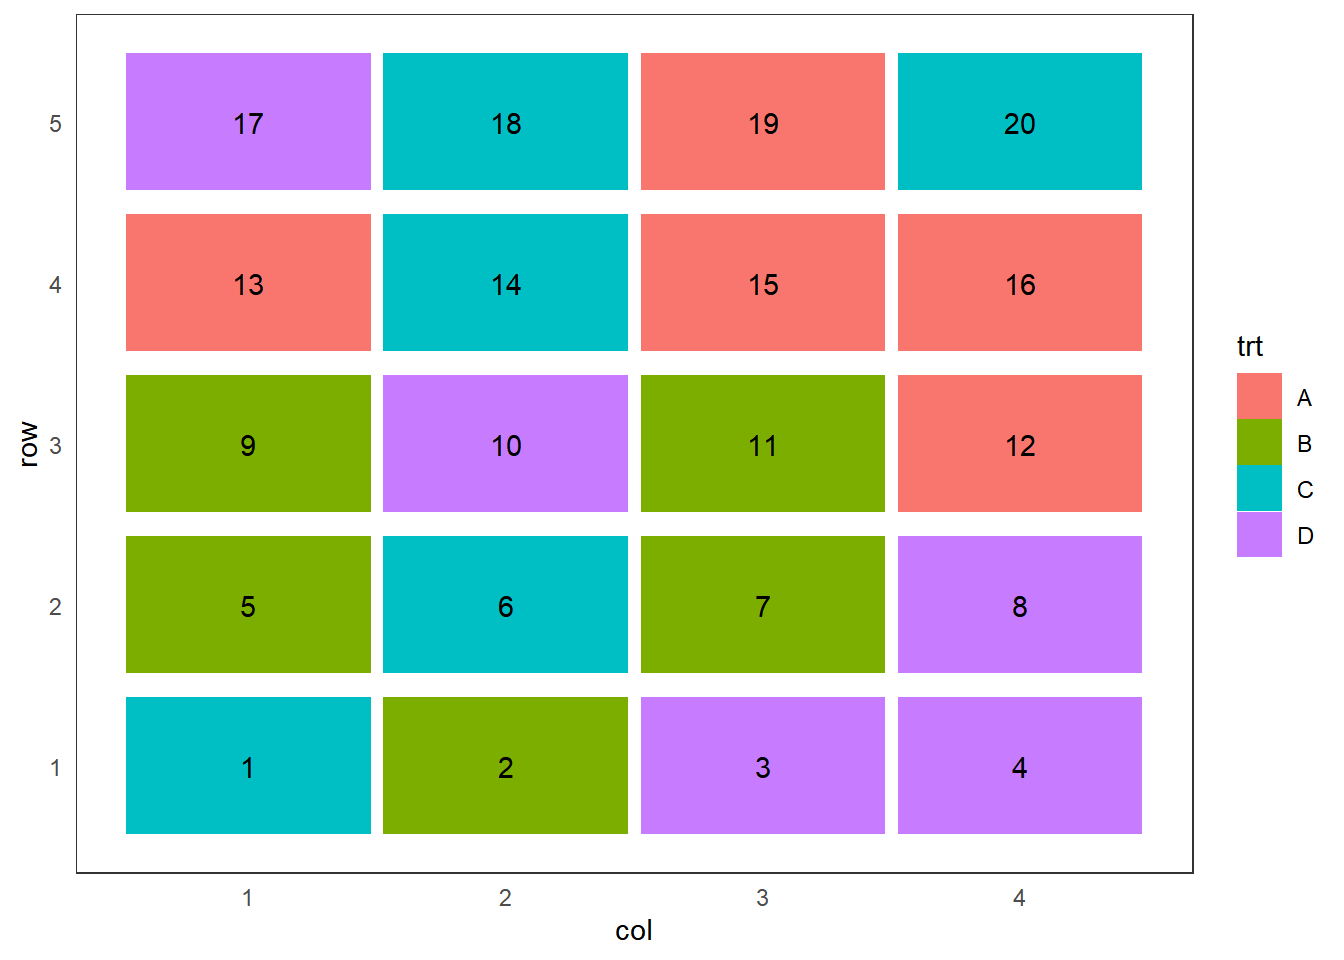
\includegraphics{_main_files/figure-latex/unnamed-chunk-3-1.pdf}

\begin{Shaded}
\begin{Highlighting}[]
\SpecialCharTok{\textgreater{}} \CommentTok{\# Para montar um croqui precisamos de um gride, definido por linhas e colunas}
\ErrorTok{\textgreater{}}\NormalTok{ delineamento}\SpecialCharTok{$}\NormalTok{book}\SpecialCharTok{$}\NormalTok{Linha }\OtherTok{\textless{}{-}} \FunctionTok{rep}\NormalTok{(}\DecValTok{1}\SpecialCharTok{:}\DecValTok{5}\NormalTok{, }\AttributeTok{each =} \DecValTok{4}\NormalTok{)}
\SpecialCharTok{\textgreater{}}\NormalTok{ delineamento}\SpecialCharTok{$}\NormalTok{book}\SpecialCharTok{$}\NormalTok{Coluna }\OtherTok{\textless{}{-}} \FunctionTok{rep}\NormalTok{(}\DecValTok{1}\SpecialCharTok{:}\DecValTok{4}\NormalTok{, }\AttributeTok{times =} \DecValTok{5}\NormalTok{)}
\SpecialCharTok{\textgreater{}} 
\ErrorTok{\textgreater{}}\NormalTok{ delineamento}\SpecialCharTok{$}\NormalTok{book}
\end{Highlighting}
\end{Shaded}

\begin{verbatim}
   plots r trt Linha Coluna
1      1 1   C     1      1
2      2 1   B     1      2
3      3 1   D     1      3
4      4 2   D     1      4
5      5 2   B     2      1
6      6 2   C     2      2
7      7 3   B     2      3
8      8 3   D     2      4
9      9 4   B     3      1
10    10 4   D     3      2
11    11 5   B     3      3
12    12 1   A     3      4
13    13 2   A     4      1
14    14 3   C     4      2
15    15 3   A     4      3
16    16 4   A     4      4
17    17 5   D     5      1
18    18 4   C     5      2
19    19 5   A     5      3
20    20 5   C     5      4
\end{verbatim}

\textbf{Importando dados de excel .xlsx}

\begin{Shaded}
\begin{Highlighting}[]
\SpecialCharTok{\textgreater{}} \CommentTok{\#Deve{-}se importar os arquivos .xlsx para o Rstudio}
\ErrorTok{\textgreater{}} \FunctionTok{library}\NormalTok{(readxl)}
\SpecialCharTok{\textgreater{}}\NormalTok{ dados1 }\OtherTok{\textless{}{-}} \FunctionTok{read\_xlsx}\NormalTok{(}\StringTok{"dados/aula2.2.xlsx"}\NormalTok{)}
\SpecialCharTok{\textgreater{}} 
\ErrorTok{\textgreater{}}\NormalTok{ knitr}\SpecialCharTok{::}\FunctionTok{kable}\NormalTok{(dados1)}
\end{Highlighting}
\end{Shaded}

\begin{tabular}{l|r}
\hline
trat & y\\
\hline
A & 25\\
\hline
A & 26\\
\hline
A & 20\\
\hline
A & 23\\
\hline
A & 21\\
\hline
B & 31\\
\hline
B & 25\\
\hline
B & 28\\
\hline
B & 27\\
\hline
B & 24\\
\hline
C & 22\\
\hline
C & 26\\
\hline
C & 28\\
\hline
C & 25\\
\hline
C & 29\\
\hline
D & 33\\
\hline
D & 29\\
\hline
D & 31\\
\hline
D & 34\\
\hline
D & 28\\
\hline
\end{tabular}

\textbf{Análise descritiva dos dados}

\begin{Shaded}
\begin{Highlighting}[]
\SpecialCharTok{\textgreater{}} \FunctionTok{library}\NormalTok{(ggplot2)}
\SpecialCharTok{\textgreater{}} \FunctionTok{ggplot}\NormalTok{(dados1, }
\SpecialCharTok{+}        \FunctionTok{aes}\NormalTok{(}\AttributeTok{x =}\NormalTok{ trat, }
\SpecialCharTok{+}            \AttributeTok{y =}\NormalTok{ y)) }\SpecialCharTok{+}
\SpecialCharTok{+}   \FunctionTok{geom\_point}\NormalTok{() }\SpecialCharTok{+}
\SpecialCharTok{+}   \FunctionTok{geom\_point}\NormalTok{(}\AttributeTok{stat =} \StringTok{"summary"}\NormalTok{,}
\SpecialCharTok{+}              \AttributeTok{fun =}\NormalTok{ mean,}
\SpecialCharTok{+}              \AttributeTok{col =} \StringTok{"red"}\NormalTok{) }\SpecialCharTok{+}
\SpecialCharTok{+}   \FunctionTok{annotate}\NormalTok{(}\StringTok{"point"}\NormalTok{, }
\SpecialCharTok{+}            \AttributeTok{x =}\NormalTok{ dados1}\SpecialCharTok{$}\NormalTok{trat, }
\SpecialCharTok{+}            \AttributeTok{y =} \FloatTok{26.75}\NormalTok{, }
\SpecialCharTok{+}            \AttributeTok{colour =} \StringTok{"blue"}\NormalTok{) }\SpecialCharTok{+}
\SpecialCharTok{+}   \FunctionTok{xlab}\NormalTok{(}\StringTok{"tratamentos"}\NormalTok{) }\SpecialCharTok{+}
\SpecialCharTok{+}   \FunctionTok{ylab}\NormalTok{(}\StringTok{"produtividade"}\NormalTok{)}
\end{Highlighting}
\end{Shaded}

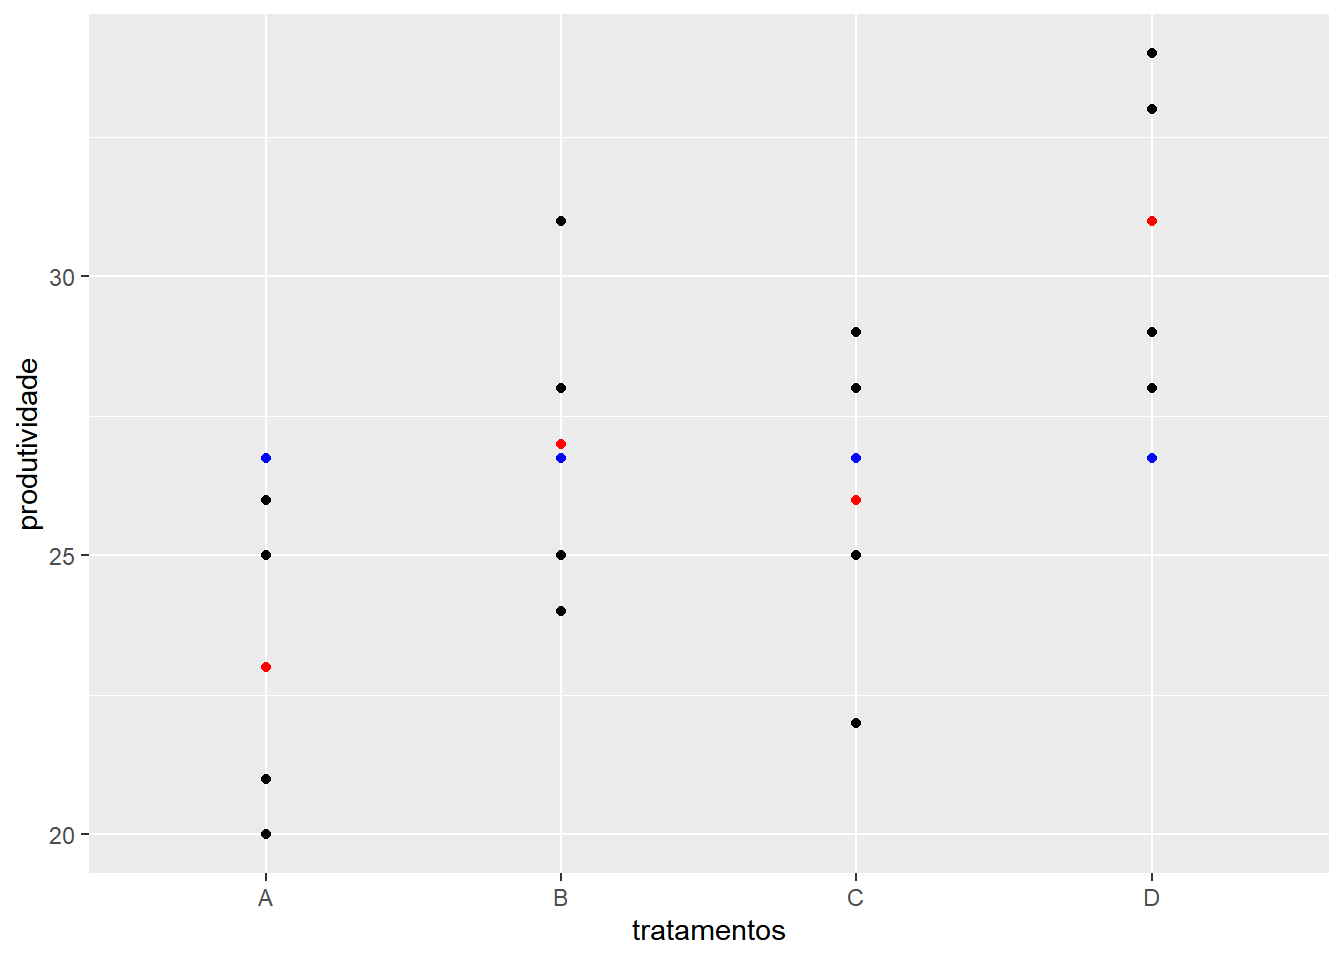
\includegraphics{_main_files/figure-latex/unnamed-chunk-5-1.pdf}

\begin{Shaded}
\begin{Highlighting}[]
\SpecialCharTok{\textgreater{}} \FunctionTok{ggplot}\NormalTok{(dados1,}
\SpecialCharTok{+}        \FunctionTok{aes}\NormalTok{(}\AttributeTok{x =}\NormalTok{ trat,}
\SpecialCharTok{+}            \AttributeTok{y =}\NormalTok{ y)) }\SpecialCharTok{+}
\SpecialCharTok{+}   \FunctionTok{geom\_boxplot}\NormalTok{()}
\end{Highlighting}
\end{Shaded}

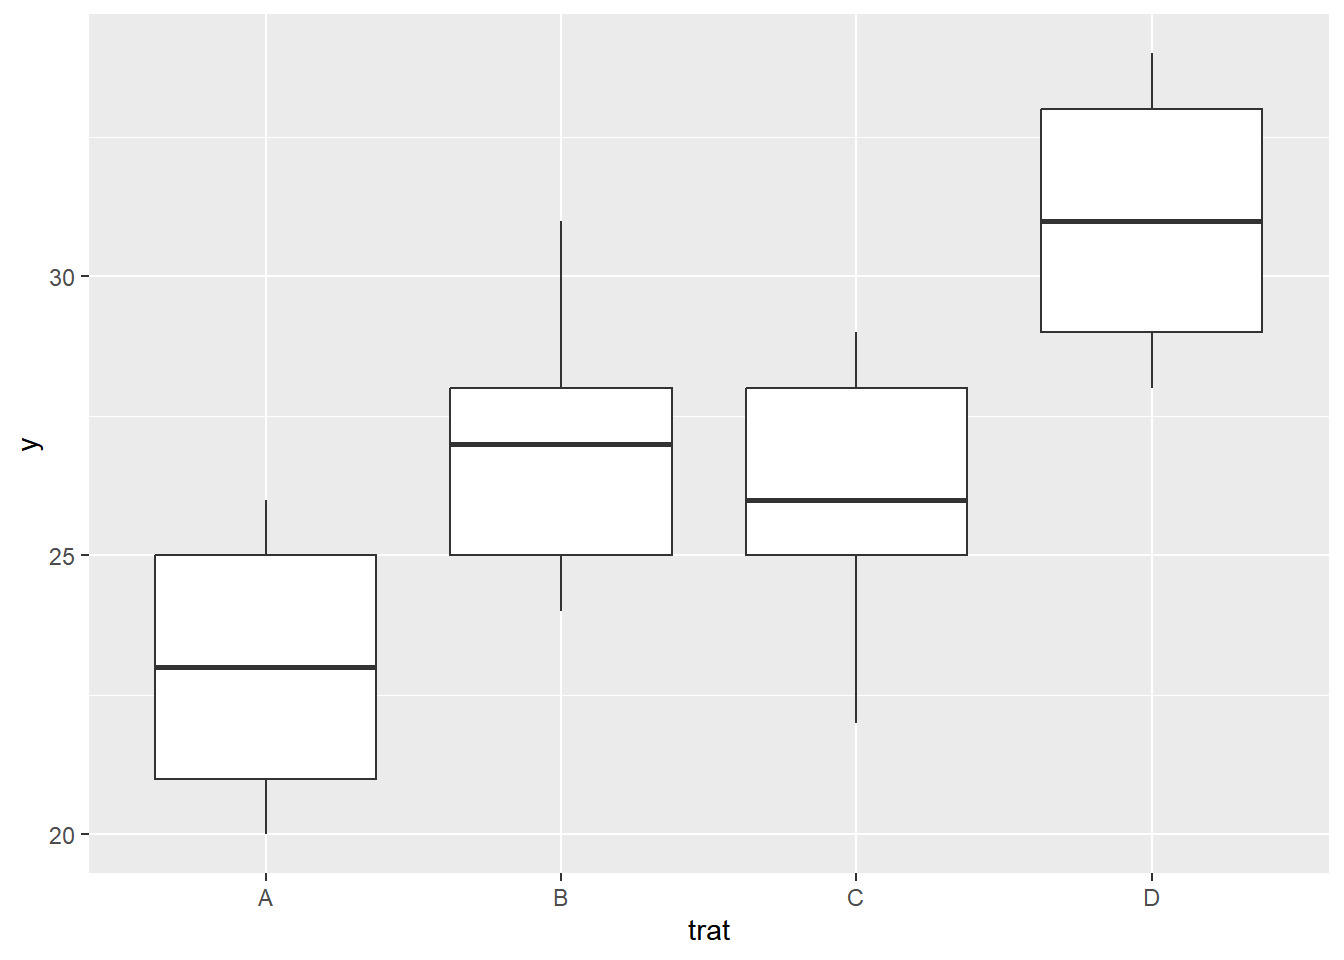
\includegraphics{_main_files/figure-latex/unnamed-chunk-5-2.pdf}

\begin{Shaded}
\begin{Highlighting}[]
\SpecialCharTok{\textgreater{}} \CommentTok{\#\textquotesingle{} \#\# Estatísticas descritivas}
\ErrorTok{\textgreater{}}\NormalTok{ n }\OtherTok{\textless{}{-}} \FunctionTok{with}\NormalTok{(dados1, }\FunctionTok{tapply}\NormalTok{(y,trat, length))}
\SpecialCharTok{\textgreater{}}\NormalTok{ soma }\OtherTok{\textless{}{-}} \FunctionTok{with}\NormalTok{(dados1, }\FunctionTok{tapply}\NormalTok{(y,trat,sum))}
\SpecialCharTok{\textgreater{}}\NormalTok{ media }\OtherTok{\textless{}{-}} \FunctionTok{with}\NormalTok{(dados1, }\FunctionTok{tapply}\NormalTok{(y,trat,mean))}
\SpecialCharTok{\textgreater{}}\NormalTok{ variancia }\OtherTok{\textless{}{-}} \FunctionTok{with}\NormalTok{(dados1, }\FunctionTok{tapply}\NormalTok{(y,trat,var))}
\SpecialCharTok{\textgreater{}}\NormalTok{ desv.padr }\OtherTok{\textless{}{-}} \FunctionTok{with}\NormalTok{(dados1, }\FunctionTok{tapply}\NormalTok{(y,trat,sd))}
\SpecialCharTok{\textgreater{}}\NormalTok{ dist.int }\OtherTok{\textless{}{-}} \FunctionTok{with}\NormalTok{(dados1, }\FunctionTok{tapply}\NormalTok{(y,trat,IQR))}
\end{Highlighting}
\end{Shaded}

\begin{Shaded}
\begin{Highlighting}[]
\SpecialCharTok{\textgreater{}} \CommentTok{\#\textquotesingle{} Criando uma função que calcula a amplitude}
\ErrorTok{\textgreater{}}\NormalTok{ f1 }\OtherTok{\textless{}{-}} \ControlFlowTok{function}\NormalTok{(x) }\FunctionTok{max}\NormalTok{(x)}\SpecialCharTok{{-}}\FunctionTok{min}\NormalTok{(x)}
\SpecialCharTok{\textgreater{}}\NormalTok{ amplitude }\OtherTok{\textless{}{-}} \FunctionTok{with}\NormalTok{(dados1, }\FunctionTok{tapply}\NormalTok{(y,trat,f1))}
\SpecialCharTok{\textgreater{}} 
\ErrorTok{\textgreater{}}\NormalTok{ resumo }\OtherTok{\textless{}{-}} \FunctionTok{rbind}\NormalTok{(n, soma, media, variancia,}
\SpecialCharTok{+}\NormalTok{                 desv.padr, amplitude,dist.int)}
\SpecialCharTok{\textgreater{}} \FunctionTok{rownames}\NormalTok{(resumo) }\OtherTok{\textless{}{-}} \FunctionTok{c}\NormalTok{(}\StringTok{"n"}\NormalTok{, }\StringTok{"Soma"}\NormalTok{, }\StringTok{"Média"}\NormalTok{, }
\SpecialCharTok{+}                       \StringTok{"Variância"}\NormalTok{, }\StringTok{"Desvio{-}padrão"}\NormalTok{, }
\SpecialCharTok{+}                       \StringTok{"Amplitude"}\NormalTok{, }\StringTok{"Amplitude Interquartílica"}\NormalTok{)}
\SpecialCharTok{\textgreater{}} \FunctionTok{round}\NormalTok{(resumo,}\DecValTok{3}\NormalTok{)}
\end{Highlighting}
\end{Shaded}

\begin{verbatim}
                               A       B       C      D
n                           5.00   5.000   5.000   5.00
Soma                      115.00 135.000 130.000 155.00
Média                      23.00  27.000  26.000  31.00
Variância                   6.50   7.500   7.500   6.50
Desvio-padrão               2.55   2.739   2.739   2.55
Amplitude                   6.00   7.000   7.000   6.00
Amplitude Interquartílica   4.00   3.000   3.000   4.00
\end{verbatim}

\textbf{Análise da variância (ANOVA)}

\begin{Shaded}
\begin{Highlighting}[]
\SpecialCharTok{\textgreater{}} \CommentTok{\#\textquotesingle{} \#\# Análise de variância  }
\ErrorTok{\textgreater{}} \CommentTok{\#\textquotesingle{} }
\ErrorTok{\textgreater{}} \CommentTok{\#\textquotesingle{} $H\_0$: $\textbackslash{}mu\_1 = \textbackslash{}mu\_2 = \textbackslash{}mu\_3 = \textbackslash{}mu\_4$ *versus* }
\ErrorTok{\textgreater{}} \CommentTok{\#\textquotesingle{} $H\_1:$ Pelo menos duas médias de tratamentos diferem entre si.}
\ErrorTok{\textgreater{}} \CommentTok{\#\textquotesingle{} }
\ErrorTok{\textgreater{}}\NormalTok{ modelo }\OtherTok{\textless{}{-}} \FunctionTok{aov}\NormalTok{(y }\SpecialCharTok{\textasciitilde{}}\NormalTok{ trat, dados1)}
\SpecialCharTok{\textgreater{}} \FunctionTok{anova}\NormalTok{(modelo)}
\end{Highlighting}
\end{Shaded}

\begin{verbatim}
Analysis of Variance Table

Response: y
          Df Sum Sq Mean Sq F value   Pr(>F)   
trat       3 163.75  54.583  7.7976 0.001976 **
Residuals 16 112.00   7.000                    
---
Signif. codes:  0 '***' 0.001 '**' 0.01 '*' 0.05 '.' 0.1 ' ' 1
\end{verbatim}

\hypertarget{exercicuxedos-2}{%
\section{Exercicíos}\label{exercicuxedos-2}}

\begin{enumerate}
\def\labelenumi{\arabic{enumi})}
\tightlist
\item
  Os dados apresentados na Tabela 1 são referentes ao peso de espigas de milho, em kg/10m², em cada parcela (10 m²). São apresentados os dados de 5 genótipos avaliados em um delineamento inteiramente casualizado (DIC) com 4 repetições.
\end{enumerate}

\begin{longtable}[]{@{}lllll@{}}
\toprule()
Genótipos & I & II & III & IV \\
\midrule()
\endhead
A & 5,95 & 6,21 & 5,40 & 5,18 \\
B & 5,07 & 6,71 & 5,46 & 4,98 \\
C & 4,82 & 5,11 & 4,68 & 4,52 \\
D & 3,87 & 4,16 & 4,11 & 4,84 \\
E & 5,53 & 5,82 & 4,29 & 4,70 \\
\bottomrule()
\end{longtable}

Considere os dados apresentados na Tabela.
a) Faça um possível croqui de instalação para um novo experimento com o mesmo número de tratamentos (genótipos) e de repetições;
b) Faça a análise exploratória dos dados de peso de espigas;
c) Faça a análise de variância e interprete o resultado do teste F considerando o nível de significância 5\%;

\begin{enumerate}
\def\labelenumi{\arabic{enumi})}
\setcounter{enumi}{1}
\tightlist
\item
  Em um experimento de competição de dez cultivares de arroz para avaliar a produtividade, instalado em um delineamento inteiramente casualizado, os resultados (parciais) para a ANOVA foram os seguintes:
\end{enumerate}

\begin{longtable}[]{@{}llllll@{}}
\toprule()
Fonte & GL & SQ & QM & F Cal & F Tab \\
\midrule()
\endhead
cultivar & x & 17564523 & x & 9.31 & 2.39 \\
Resíduo & x & x & x & x & x \\
Total & 29 & x & x & x & x \\
\bottomrule()
\end{longtable}

\begin{enumerate}
\def\labelenumi{\alph{enumi})}
\item
  Complete o quadro da ANOVA
\item
  Com base no resultado da ANOVA escreva as hipóteses e a conclusão
\end{enumerate}

\hypertarget{comparauxe7uxe3o-de-muxe9dias}{%
\chapter{Comparação de médias}\label{comparauxe7uxe3o-de-muxe9dias}}

\hypertarget{teste-de-tukey}{%
\section{Teste de Tukey}\label{teste-de-tukey}}

\hypertarget{aplicauxe7uxe3o-no-r-studio-3}{%
\subsection{Aplicação no R studio}\label{aplicauxe7uxe3o-no-r-studio-3}}

\hypertarget{exercicuxedos-3}{%
\subsection{Exercicíos}\label{exercicuxedos-3}}

\hypertarget{teste-de-duncan}{%
\section{Teste de Duncan}\label{teste-de-duncan}}

\hypertarget{aplicauxe7uxe3o-no-r-studio-4}{%
\subsection{Aplicação no R studio}\label{aplicauxe7uxe3o-no-r-studio-4}}

\hypertarget{exercicuxedos-4}{%
\subsection{Exercicíos}\label{exercicuxedos-4}}

\hypertarget{teste-de-dunnett}{%
\section{Teste de Dunnett}\label{teste-de-dunnett}}

\hypertarget{aplicauxe7uxe3o-no-r-studio-5}{%
\subsection{Aplicação no R studio}\label{aplicauxe7uxe3o-no-r-studio-5}}

\hypertarget{exercicuxedos-5}{%
\subsection{Exercicíos}\label{exercicuxedos-5}}

\hypertarget{teste-de-scheffuxe9}{%
\section{Teste de Scheffé}\label{teste-de-scheffuxe9}}

\hypertarget{aplicauxe7uxe3o-no-r-studio-6}{%
\subsection{Aplicação no R studio}\label{aplicauxe7uxe3o-no-r-studio-6}}

\hypertarget{exercicuxedos-6}{%
\subsection{Exercicíos}\label{exercicuxedos-6}}

\hypertarget{contrastes-ortogonais}{%
\section{Contrastes ortogonais}\label{contrastes-ortogonais}}

\hypertarget{aplicauxe7uxe3o-no-r-studio-7}{%
\subsection{Aplicação no R studio}\label{aplicauxe7uxe3o-no-r-studio-7}}

\hypertarget{exercicuxedos-7}{%
\subsection{Exercicíos}\label{exercicuxedos-7}}

\hypertarget{regressuxe3o-polinomial}{%
\chapter{Regressão polinomial}\label{regressuxe3o-polinomial}}

\hypertarget{anova}{%
\section{Anova}\label{anova}}

\hypertarget{aplicauxe7uxe3o-no-r-studio-8}{%
\section{Aplicação no R studio}\label{aplicauxe7uxe3o-no-r-studio-8}}

\hypertarget{exercicuxedos-8}{%
\section{Exercicíos}\label{exercicuxedos-8}}

\hypertarget{delineamento-em-blocos-casualizados}{%
\chapter{Delineamento em blocos casualizados}\label{delineamento-em-blocos-casualizados}}

\hypertarget{anova-1}{%
\section{Anova}\label{anova-1}}

\hypertarget{aplicauxe7uxe3o-no-r-studio-9}{%
\section{Aplicação no R studio}\label{aplicauxe7uxe3o-no-r-studio-9}}

\hypertarget{exercicuxedos-9}{%
\section{Exercicíos}\label{exercicuxedos-9}}

\hypertarget{delineamento-quadrado-latino}{%
\chapter{Delineamento quadrado latino}\label{delineamento-quadrado-latino}}

\hypertarget{anova-2}{%
\section{Anova}\label{anova-2}}

\hypertarget{aplicauxe7uxe3o-no-r-studio-10}{%
\section{Aplicação no R studio}\label{aplicauxe7uxe3o-no-r-studio-10}}

\hypertarget{exercicuxedos-10}{%
\section{Exercicíos}\label{exercicuxedos-10}}

\hypertarget{experimento-fatorial}{%
\chapter{Experimento fatorial}\label{experimento-fatorial}}

\hypertarget{anova-3}{%
\section{Anova}\label{anova-3}}

\hypertarget{aplicauxe7uxe3o-no-r-studio-11}{%
\section{Aplicação no R studio}\label{aplicauxe7uxe3o-no-r-studio-11}}

\hypertarget{exercicuxedos-11}{%
\section{Exercicíos}\label{exercicuxedos-11}}

\hypertarget{experimento-em-parcelas-subdivididas-e-em-faixas}{%
\chapter{Experimento em parcelas subdivididas e em faixas}\label{experimento-em-parcelas-subdivididas-e-em-faixas}}

\hypertarget{anova-4}{%
\section{Anova}\label{anova-4}}

\hypertarget{aplicauxe7uxe3o-no-r-studio-12}{%
\section{Aplicação no R studio}\label{aplicauxe7uxe3o-no-r-studio-12}}

\hypertarget{exercicuxedos-12}{%
\section{Exercicíos}\label{exercicuxedos-12}}

\end{document}
